\documentclass[twoside]{book}

% Packages required by doxygen
\usepackage{fixltx2e}
\usepackage{calc}
\usepackage{doxygen}
\usepackage[export]{adjustbox} % also loads graphicx
\usepackage{graphicx}
\usepackage[utf8]{inputenc}
\usepackage{makeidx}
\usepackage{multicol}
\usepackage{multirow}
\PassOptionsToPackage{warn}{textcomp}
\usepackage{textcomp}
\usepackage[nointegrals]{wasysym}
\usepackage[table]{xcolor}

% Font selection
\usepackage[T1]{fontenc}
\usepackage[scaled=.90]{helvet}
\usepackage{courier}
\usepackage{amssymb}
\usepackage{sectsty}
\renewcommand{\familydefault}{\sfdefault}
\allsectionsfont{%
  \fontseries{bc}\selectfont%
  \color{darkgray}%
}
\renewcommand{\DoxyLabelFont}{%
  \fontseries{bc}\selectfont%
  \color{darkgray}%
}
\newcommand{\+}{\discretionary{\mbox{\scriptsize$\hookleftarrow$}}{}{}}

% Page & text layout
\usepackage{geometry}
\geometry{%
  a4paper,%
  top=2.5cm,%
  bottom=2.5cm,%
  left=2.5cm,%
  right=2.5cm%
}
\tolerance=750
\hfuzz=15pt
\hbadness=750
\setlength{\emergencystretch}{15pt}
\setlength{\parindent}{0cm}
\setlength{\parskip}{3ex plus 2ex minus 2ex}
\makeatletter
\renewcommand{\paragraph}{%
  \@startsection{paragraph}{4}{0ex}{-1.0ex}{1.0ex}{%
    \normalfont\normalsize\bfseries\SS@parafont%
  }%
}
\renewcommand{\subparagraph}{%
  \@startsection{subparagraph}{5}{0ex}{-1.0ex}{1.0ex}{%
    \normalfont\normalsize\bfseries\SS@subparafont%
  }%
}
\makeatother

% Headers & footers
\usepackage{fancyhdr}
\pagestyle{fancyplain}
\fancyhead[LE]{\fancyplain{}{\bfseries\thepage}}
\fancyhead[CE]{\fancyplain{}{}}
\fancyhead[RE]{\fancyplain{}{\bfseries\leftmark}}
\fancyhead[LO]{\fancyplain{}{\bfseries\rightmark}}
\fancyhead[CO]{\fancyplain{}{}}
\fancyhead[RO]{\fancyplain{}{\bfseries\thepage}}
\fancyfoot[LE]{\fancyplain{}{}}
\fancyfoot[CE]{\fancyplain{}{}}
\fancyfoot[RE]{\fancyplain{}{\bfseries\scriptsize Generated by Doxygen }}
\fancyfoot[LO]{\fancyplain{}{\bfseries\scriptsize Generated by Doxygen }}
\fancyfoot[CO]{\fancyplain{}{}}
\fancyfoot[RO]{\fancyplain{}{}}
\renewcommand{\footrulewidth}{0.4pt}
\renewcommand{\chaptermark}[1]{%
  \markboth{#1}{}%
}
\renewcommand{\sectionmark}[1]{%
  \markright{\thesection\ #1}%
}

% Indices & bibliography
\usepackage{natbib}
\usepackage[titles]{tocloft}
\setcounter{tocdepth}{3}
\setcounter{secnumdepth}{5}
\makeindex

% Custom commands
\newcommand{\clearemptydoublepage}{%
  \newpage{\pagestyle{empty}\cleardoublepage}%
}

\usepackage{caption}
\captionsetup{labelsep=space,justification=centering,font={bf},singlelinecheck=off,skip=4pt,position=top}

%===== C O N T E N T S =====

\begin{document}

% Titlepage & ToC
\pagenumbering{alph}
\begin{titlepage}
\vspace*{7cm}
\begin{center}%
{\Large Map Editor }\\
\vspace*{1cm}
{\large Generated by Doxygen 1.8.13}\\
\end{center}
\end{titlepage}
\clearemptydoublepage
\pagenumbering{roman}
\tableofcontents
\clearemptydoublepage
\pagenumbering{arabic}

%--- Begin generated contents ---
\chapter{Hierarchical Index}
\section{Class Hierarchy}
This inheritance list is sorted roughly, but not completely, alphabetically\+:\begin{DoxyCompactList}
\item \contentsline{section}{Game}{\pageref{class_game}}{}
\item Sprite\begin{DoxyCompactList}
\item \contentsline{section}{Abstract\+\_\+\+Field}{\pageref{class_abstract___field}}{}
\begin{DoxyCompactList}
\item \contentsline{section}{Manager}{\pageref{class_manager}}{}
\item \contentsline{section}{Map\+\_\+\+Net}{\pageref{class_map___net}}{}
\end{DoxyCompactList}
\end{DoxyCompactList}
\item \contentsline{section}{Texture\+\_\+\+Manager}{\pageref{class_texture___manager}}{}
\end{DoxyCompactList}

\chapter{Class Index}
\section{Class List}
Here are the classes, structs, unions and interfaces with brief descriptions\+:\begin{DoxyCompactList}
\item\contentsline{section}{\textbf{ Abstract\+\_\+\+Field} }{\pageref{class_abstract___field}}{}
\item\contentsline{section}{\textbf{ Game} }{\pageref{class_game}}{}
\item\contentsline{section}{\textbf{ Manager} }{\pageref{class_manager}}{}
\item\contentsline{section}{\textbf{ Map\+\_\+\+Net} }{\pageref{class_map___net}}{}
\item\contentsline{section}{\textbf{ Texture\+\_\+\+Manager} \\*This class allows you to use textures in the program }{\pageref{class_texture___manager}}{}
\end{DoxyCompactList}

\chapter{File Index}
\section{File List}
Here is a list of all documented files with brief descriptions\+:\begin{DoxyCompactList}
\item\contentsline{section}{\textbf{ main\+\_\+header.\+hpp} \\*The header file which unites any other useful headers }{\pageref{main__header_8hpp}}{}
\end{DoxyCompactList}

\chapter{Class Documentation}
\section{Abstract\+\_\+\+Field Class Reference}
\label{class_abstract___field}\index{Abstract\+\_\+\+Field@{Abstract\+\_\+\+Field}}


Inheritance diagram for Abstract\+\_\+\+Field\+:
\nopagebreak
\begin{figure}[H]
\begin{center}
\leavevmode
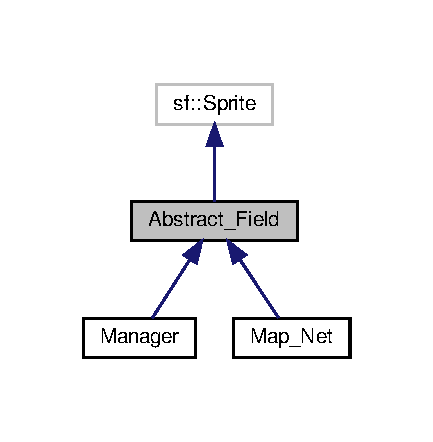
\includegraphics[width=208pt]{class_abstract___field__inherit__graph}
\end{center}
\end{figure}


Collaboration diagram for Abstract\+\_\+\+Field\+:
\nopagebreak
\begin{figure}[H]
\begin{center}
\leavevmode
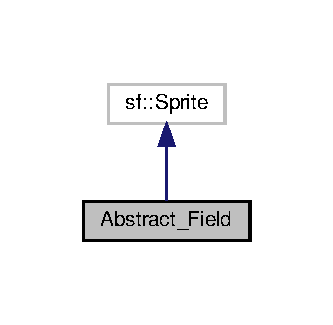
\includegraphics[width=160pt]{class_abstract___field__coll__graph}
\end{center}
\end{figure}
\subsection*{Public Member Functions}
\begin{DoxyCompactItemize}
\item 
\mbox{\label{class_abstract___field_a97f869f349e8015e9d75b74db9cd80f1}} 
{\bfseries Abstract\+\_\+\+Field} (float x, float y) noexcept
\item 
\mbox{\label{class_abstract___field_ad0e859cfd1a759a8289f36b2b2d6595e}} 
{\bfseries Abstract\+\_\+\+Field} (float x, float y, \textbf{ Texture\+\_\+\+Manager\+::\+ID} id) noexcept
\item 
\mbox{\label{class_abstract___field_abc7aa6d6b6160a275da6d1cf1f842a95}} 
void {\bfseries set\+\_\+texture} (\textbf{ Texture\+\_\+\+Manager\+::\+ID} id) noexcept
\item 
\mbox{\label{class_abstract___field_a3798b5a3d66436e7387577252e8a4ad7}} 
void {\bfseries set\+\_\+transparent} (bool transparent) noexcept
\item 
\mbox{\label{class_abstract___field_aeab84f13667c01a0270883f7ef3b95a5}} 
bool {\bfseries get\+\_\+transparent} (void) const noexcept
\item 
\mbox{\label{class_abstract___field_aa3a501afd173d5e441481e3bc3102490}} 
virtual int {\bfseries handle\+\_\+\+Mouse\+\_\+\+Pressed} (float x, float y) const noexcept
\item 
\mbox{\label{class_abstract___field_a5403c00346a45dff0af4a13a2d932111}} 
virtual bool {\bfseries is\+\_\+on\+\_\+\+Mouse} (float x, float y) const noexcept
\item 
\mbox{\label{class_abstract___field_a6f27798053ffbe86d89e520c3ba1eac0}} 
virtual void {\bfseries render} (sf\+::\+Render\+Window \&window) const noexcept
\end{DoxyCompactItemize}


The documentation for this class was generated from the following files\+:\begin{DoxyCompactItemize}
\item 
\textbf{ main\+\_\+header.\+hpp}\item 
Buttons.\+cpp\end{DoxyCompactItemize}

\section{Game Class Reference}
\label{class_game}\index{Game@{Game}}


Collaboration diagram for Game\+:
\nopagebreak
\begin{figure}[H]
\begin{center}
\leavevmode
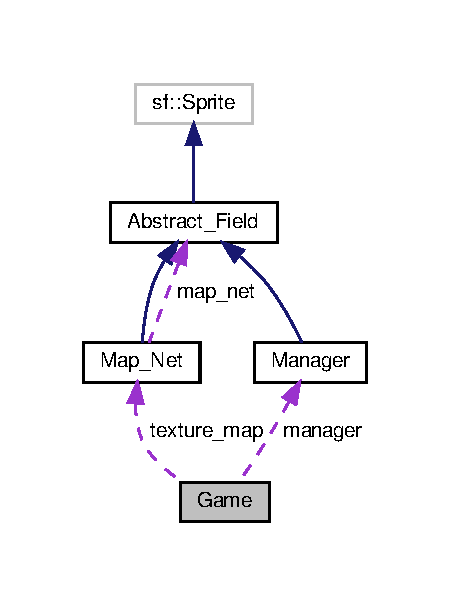
\includegraphics[width=216pt]{class_game__coll__graph}
\end{center}
\end{figure}
\subsection*{Public Member Functions}
\begin{DoxyCompactItemize}
\item 
\mbox{\label{class_game_a5bc07cf8947858f32637943836cc6f8e}} 
{\bfseries Game} (int width, int height)
\item 
\mbox{\label{class_game_a1e5138ddc86047f2cb1171758a583df1}} 
void {\bfseries construct} (void) noexcept
\item 
\mbox{\label{class_game_a46165f87463fa8114fa44596ced90dbd}} 
void {\bfseries run} (void)
\item 
\mbox{\label{class_game_aee38b1aa52dba2855f2457d22b3df13f}} 
void {\bfseries render} (void)
\item 
\mbox{\label{class_game_a36bf09723c976fe477bc774cc1d03b3f}} 
void {\bfseries update} (void)
\item 
\mbox{\label{class_game_a16c9b0feaf6b088bdcd591c731e68981}} 
void {\bfseries load\+\_\+map} (void)
\item 
\mbox{\label{class_game_a8bf297e096e1818ee04490704dd2aa47}} 
void {\bfseries handle\+\_\+\+Events} (void)
\item 
\mbox{\label{class_game_a33ba12022b4e9211e47231a2cb7420a8}} 
void {\bfseries load\+\_\+textures} (void)
\item 
\mbox{\label{class_game_a8ee964a0e77476e2755be37868c67db6}} 
void {\bfseries preprocessing} (void)
\item 
\mbox{\label{class_game_ab557af9fcbd7bf45c3bd98ba6014b79b}} 
void {\bfseries make\+\_\+default\+\_\+map} (void) noexcept
\item 
\mbox{\label{class_game_a6a0260cb97b25515e10b7fd2239780cc}} 
void {\bfseries handle\+\_\+zoom} (float delta) noexcept
\item 
\mbox{\label{class_game_ae37df91bc39bf902d49477d2023601a7}} 
void {\bfseries handle\+\_\+scrolling} (float x, float y) noexcept
\item 
\mbox{\label{class_game_aa98202aec960f630979076cfdd1754a8}} 
sf\+::\+Vector2i {\bfseries calculate\+\_\+coordinates} (void) const noexcept
\end{DoxyCompactItemize}
\subsection*{Public Attributes}
\begin{DoxyCompactItemize}
\item 
\mbox{\label{class_game_a7f7bcbfabe1f934a35b4b2ebb07ab081}} 
\textbf{ Map\+\_\+\+Net} {\bfseries texture\+\_\+map}
\item 
\mbox{\label{class_game_a793d916f26e5b18585a924f0b04d3d29}} 
sf\+::\+Vector2i {\bfseries offset}
\item 
\mbox{\label{class_game_a8692b6957cee6766cb8dea1120e26b52}} 
sf\+::\+Vector2i {\bfseries scale\+\_\+offset}
\item 
\mbox{\label{class_game_aabe9e45119ae00b3b11cff84e10d15ae}} 
double {\bfseries scale} = 1
\item 
\mbox{\label{class_game_a223de215aeb661cd423ac145756cc730}} 
sf\+::\+Render\+Window {\bfseries window}
\item 
\mbox{\label{class_game_ac136054a272ae71ed3697acc58ee13a0}} 
sf\+::\+Vector2f {\bfseries window\+\_\+size}
\item 
\mbox{\label{class_game_a72739bdd7a7159a83394be25d7e116d6}} 
sf\+::\+View {\bfseries view}
\item 
\mbox{\label{class_game_afaa30a69a82e00c28792bb472b8dd8d9}} 
\textbf{ Manager} {\bfseries manager}
\end{DoxyCompactItemize}


The documentation for this class was generated from the following files\+:\begin{DoxyCompactItemize}
\item 
\textbf{ main\+\_\+header.\+hpp}\item 
Game\+\_\+\+Class.\+cpp\end{DoxyCompactItemize}

\section{Manager Class Reference}
\label{class_manager}\index{Manager@{Manager}}


Inheritance diagram for Manager\+:
\nopagebreak
\begin{figure}[H]
\begin{center}
\leavevmode
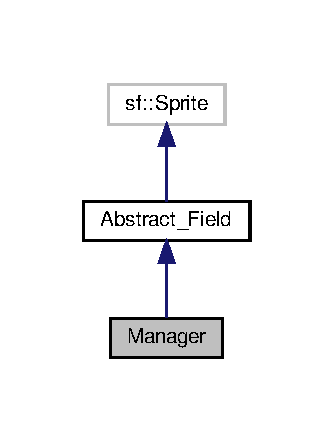
\includegraphics[width=160pt]{class_manager__inherit__graph}
\end{center}
\end{figure}


Collaboration diagram for Manager\+:
\nopagebreak
\begin{figure}[H]
\begin{center}
\leavevmode
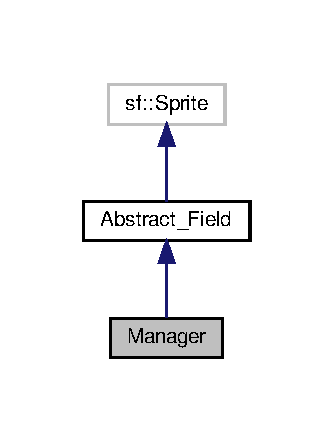
\includegraphics[width=160pt]{class_manager__coll__graph}
\end{center}
\end{figure}
\subsection*{Public Member Functions}
\begin{DoxyCompactItemize}
\item 
\mbox{\label{class_manager_a96cd1ec402e2c7eae1bcfba02e2b98b6}} 
{\bfseries Manager} (int number) noexcept
\item 
\mbox{\label{class_manager_a50645ccfb34fbf2ca5a2cb2d71b6a4cf}} 
{\bfseries Manager} (float x, float y) noexcept
\item 
\mbox{\label{class_manager_afa63bf1660484bb7e0f59e8442463233}} 
{\bfseries Manager} (float x, float y, \textbf{ Texture\+\_\+\+Manager\+::\+ID} id) noexcept
\item 
\mbox{\label{class_manager_a7b8a0c6a669ac52cba99504a55fee9ee}} 
virtual int {\bfseries handle\+\_\+\+Mouse\+\_\+\+Pressed} (float x, float y) const noexcept override
\item 
\mbox{\label{class_manager_a6831593059b3466ef04dbaf49fc86a26}} 
virtual void {\bfseries render} (sf\+::\+Render\+Window \&window) const noexcept override
\item 
\mbox{\label{class_manager_a02ef98b2d31dd2a0dc9904f851683e4b}} 
void {\bfseries insert} (\textbf{ Abstract\+\_\+\+Field} $\ast$new\+\_\+field) noexcept
\end{DoxyCompactItemize}
\subsection*{Public Attributes}
\begin{DoxyCompactItemize}
\item 
\mbox{\label{class_manager_a68fec7e7b354db503dd062da7bc03b34}} 
std\+::vector$<$ \textbf{ Abstract\+\_\+\+Field} $\ast$ $>$ {\bfseries array}
\end{DoxyCompactItemize}


The documentation for this class was generated from the following files\+:\begin{DoxyCompactItemize}
\item 
\textbf{ main\+\_\+header.\+hpp}\item 
Buttons.\+cpp\end{DoxyCompactItemize}

\section{Map\+\_\+\+Net Class Reference}
\label{class_map___net}\index{Map\+\_\+\+Net@{Map\+\_\+\+Net}}


Inheritance diagram for Map\+\_\+\+Net\+:
\nopagebreak
\begin{figure}[H]
\begin{center}
\leavevmode
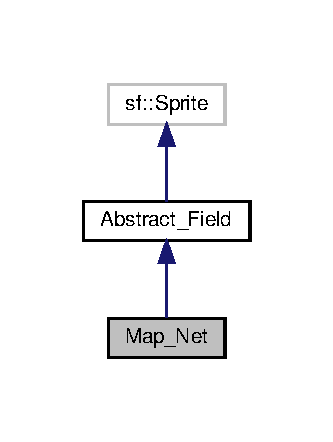
\includegraphics[width=160pt]{class_map___net__inherit__graph}
\end{center}
\end{figure}


Collaboration diagram for Map\+\_\+\+Net\+:
\nopagebreak
\begin{figure}[H]
\begin{center}
\leavevmode
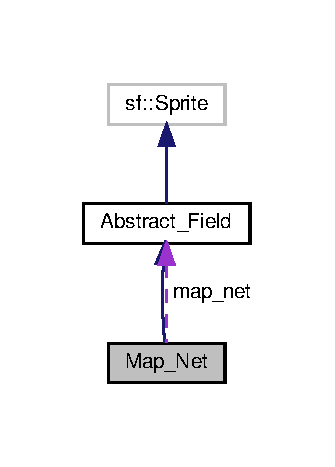
\includegraphics[width=161pt]{class_map___net__coll__graph}
\end{center}
\end{figure}
\subsection*{Public Member Functions}
\begin{DoxyCompactItemize}
\item 
\mbox{\label{class_map___net_a72098dca512b6086584c4e214c508deb}} 
void {\bfseries set\+\_\+settings} (size\+\_\+t left\+\_\+edge, size\+\_\+t upper\+\_\+edge, size\+\_\+t width, size\+\_\+t height) noexcept
\item 
\mbox{\label{class_map___net_a0ba6c77ccedf4b8bb2102b15280c86f8}} 
virtual int {\bfseries handle\+\_\+\+Mouse\+\_\+\+Pressed} (float x, float y) const noexcept override
\item 
\mbox{\label{class_map___net_a8fedbbe40c44d1a4b246b1411e67ed00}} 
virtual bool {\bfseries is\+\_\+on\+\_\+\+Mouse} (float x, float y) const noexcept override
\item 
\mbox{\label{class_map___net_a0ca23d4daf65cf43570dbb48daaf915e}} 
virtual void {\bfseries render} (sf\+::\+Render\+Window \&window) const noexcept override
\end{DoxyCompactItemize}
\subsection*{Public Attributes}
\begin{DoxyCompactItemize}
\item 
\mbox{\label{class_map___net_ab5a79d93310eda767ec819bdfedba1c1}} 
size\+\_\+t {\bfseries texture\+\_\+size} = 32
\item 
\mbox{\label{class_map___net_a4a91668f7ca122ce7aac8283cca3dca9}} 
size\+\_\+t {\bfseries left\+\_\+edge} = 30
\item 
\mbox{\label{class_map___net_a881563a0a6a643caef6c94a06f5733ca}} 
size\+\_\+t {\bfseries upper\+\_\+edge} = 30
\item 
\mbox{\label{class_map___net_a21ece0792b6162c518566756afe67bd1}} 
size\+\_\+t {\bfseries width} = 60
\item 
\mbox{\label{class_map___net_a9fd41f4e69151c0042e564b1b98cc607}} 
size\+\_\+t {\bfseries height} = 60
\item 
\mbox{\label{class_map___net_aea7e8999905efe6d88c6506f7b7839d1}} 
\textbf{ Abstract\+\_\+\+Field} $\ast$$\ast$ {\bfseries map\+\_\+net}
\end{DoxyCompactItemize}


The documentation for this class was generated from the following files\+:\begin{DoxyCompactItemize}
\item 
\textbf{ main\+\_\+header.\+hpp}\item 
Buttons.\+cpp\end{DoxyCompactItemize}

\section{Texture\+\_\+\+Manager Class Reference}
\label{class_texture___manager}\index{Texture\+\_\+\+Manager@{Texture\+\_\+\+Manager}}


This class allows you to use textures in the program.  




{\ttfamily \#include $<$main\+\_\+header.\+hpp$>$}

\subsection*{Public Types}
\begin{DoxyCompactItemize}
\item 
enum \textbf{ ID} \{ \newline
{\bfseries logo}, 
{\bfseries castle}, 
{\bfseries map}, 
{\bfseries grass}, 
\newline
{\bfseries forest\+\_\+1}, 
\textbf{ texture\+\_\+number}
 \}\begin{DoxyCompactList}\small\item\em Possible names-\/identificators of pictures. \end{DoxyCompactList}
\end{DoxyCompactItemize}
\subsection*{Public Member Functions}
\begin{DoxyCompactItemize}
\item 
void \textbf{ load} (\textbf{ Texture\+\_\+\+Manager\+::\+ID} id, const char $\ast$file\+\_\+name)
\item 
sf\+::\+Texture \& \textbf{ get\+\_\+texture} (\textbf{ Texture\+\_\+\+Manager\+::\+ID} id) const noexcept
\end{DoxyCompactItemize}


\subsection{Detailed Description}
This class allows you to use textures in the program. 

\begin{DoxyVersion}{Version}
1.\+0 
\end{DoxyVersion}
\begin{DoxyDate}{Date}
2, July, 2020 
\end{DoxyDate}
\begin{DoxyWarning}{Warning}
Many operation have asymptotics O (log n) as it uses a std\+::map.
\end{DoxyWarning}
This class has a enum with possibble names of textures. It also has a std\+::map which contains pairs I\+D-\/number -\/ unique\+\_\+ptr to the texture. 

\subsection{Member Enumeration Documentation}
\mbox{\label{class_texture___manager_ad63782cc856b6b2f5f2d5a50446ca589}} 
\index{Texture\+\_\+\+Manager@{Texture\+\_\+\+Manager}!ID@{ID}}
\index{ID@{ID}!Texture\+\_\+\+Manager@{Texture\+\_\+\+Manager}}
\subsubsection{ID}
{\footnotesize\ttfamily enum \textbf{ Texture\+\_\+\+Manager\+::\+ID}}



Possible names-\/identificators of pictures. 

\begin{DoxyEnumFields}{Enumerator}
\raisebox{\heightof{T}}[0pt][0pt]{\index{texture\+\_\+number@{texture\+\_\+number}!Texture\+\_\+\+Manager@{Texture\+\_\+\+Manager}}\index{Texture\+\_\+\+Manager@{Texture\+\_\+\+Manager}!texture\+\_\+number@{texture\+\_\+number}}}\mbox{\label{class_texture___manager_ad63782cc856b6b2f5f2d5a50446ca589a556b14f5a3303471af929dcb18cf9ca4}} 
texture\+\_\+number&Number of different texture names. \\
\hline

\end{DoxyEnumFields}

\begin{DoxyCode}
49             \{
50                 logo, castle, map,
51                 grass, forest\_1,
52                 texture_number          
53             \};
\end{DoxyCode}


\subsection{Member Function Documentation}
\mbox{\label{class_texture___manager_a0af52a4c629ad3fab88437c7ff13ef3c}} 
\index{Texture\+\_\+\+Manager@{Texture\+\_\+\+Manager}!get\+\_\+texture@{get\+\_\+texture}}
\index{get\+\_\+texture@{get\+\_\+texture}!Texture\+\_\+\+Manager@{Texture\+\_\+\+Manager}}
\subsubsection{get\+\_\+texture()}
{\footnotesize\ttfamily sf\+::\+Texture \& Texture\+\_\+\+Manager\+::get\+\_\+texture (\begin{DoxyParamCaption}\item[{\textbf{ Texture\+\_\+\+Manager\+::\+ID}}]{id }\end{DoxyParamCaption}) const\hspace{0.3cm}{\ttfamily [noexcept]}}

Gets a reference to the texture with this ID. 
\begin{DoxyParams}[1]{Parameters}
\mbox{\tt in}  & {\em id} & The identifying number of the image. Should be in enum ID. \\
\hline
\end{DoxyParams}
\begin{DoxyReturn}{Returns}
reference to the texture. 
\end{DoxyReturn}

\begin{DoxyCode}
15 \{
16     \textcolor{keywordflow}{return} *(this->Texture\_Map.find (\textcolor{keywordtype}{id})->second);
17 \}
\end{DoxyCode}
\mbox{\label{class_texture___manager_ab307261ce9f9ed3cec6a316d7e8ad40c}} 
\index{Texture\+\_\+\+Manager@{Texture\+\_\+\+Manager}!load@{load}}
\index{load@{load}!Texture\+\_\+\+Manager@{Texture\+\_\+\+Manager}}
\subsubsection{load()}
{\footnotesize\ttfamily void Texture\+\_\+\+Manager\+::load (\begin{DoxyParamCaption}\item[{\textbf{ Texture\+\_\+\+Manager\+::\+ID}}]{id,  }\item[{const char $\ast$}]{file\+\_\+name }\end{DoxyParamCaption})}

Loads an image, so it can be used further in the program. 
\begin{DoxyParams}[1]{Parameters}
\mbox{\tt in}  & {\em id} & The identifying number of the image. Should be in enum ID. \\
\hline
\mbox{\tt in}  & {\em file\+\_\+name} & The name and the path to the image. \\
\hline
\end{DoxyParams}

\begin{DoxyExceptions}{Exceptions}
{\em std\+::runtime\+\_\+error} & If there is no file with such name in the folder. \\
\hline
\end{DoxyExceptions}

\begin{DoxyCode}
22 \{
23     std::unique\_ptr <sf::Texture> unique\_texture (\textcolor{keyword}{new} sf::Texture());
24 
25     \textcolor{keywordflow}{if} (!unique\_texture->loadFromFile (file\_name))
26         \textcolor{keywordflow}{throw} std::runtime\_error (\textcolor{stringliteral}{"Failed to load file "} + std::string (file\_name));
27 
28     this->Texture\_Map.insert (std::make\_pair (\textcolor{keywordtype}{id}, std::move (unique\_texture)));
29 \}
\end{DoxyCode}


The documentation for this class was generated from the following files\+:\begin{DoxyCompactItemize}
\item 
\textbf{ main\+\_\+header.\+hpp}\item 
Textures.\+cpp\end{DoxyCompactItemize}

\chapter{File Documentation}
\section{main\+\_\+header.\+hpp File Reference}
\label{main__header_8hpp}\index{main\+\_\+header.\+hpp@{main\+\_\+header.\+hpp}}


The header file which unites any other useful headers.  


{\ttfamily \#include $<$stdlib.\+h$>$}\newline
{\ttfamily \#include $<$stdio.\+h$>$}\newline
{\ttfamily \#include $<$S\+F\+M\+L/\+Graphics.\+hpp$>$}\newline
Include dependency graph for main\+\_\+header.\+hpp\+:
\nopagebreak
\begin{figure}[H]
\begin{center}
\leavevmode
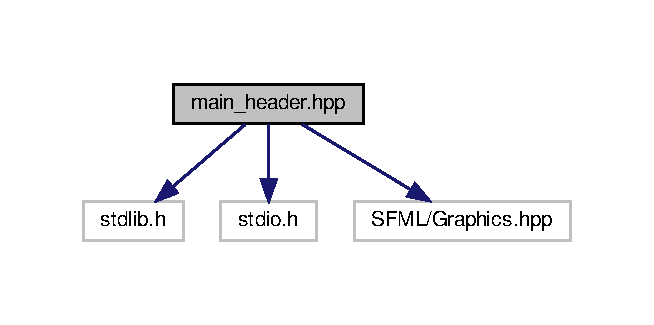
\includegraphics[width=314pt]{main__header_8hpp__incl}
\end{center}
\end{figure}
\subsection*{Classes}
\begin{DoxyCompactItemize}
\item 
class \textbf{ Texture\+\_\+\+Manager}
\begin{DoxyCompactList}\small\item\em This class allows you to use textures in the program. \end{DoxyCompactList}\item 
class \textbf{ Abstract\+\_\+\+Field}
\item 
class \textbf{ Manager}
\item 
class \textbf{ Map\+\_\+\+Net}
\item 
class \textbf{ Game}
\end{DoxyCompactItemize}
\subsection*{Variables}
\begin{DoxyCompactItemize}
\item 
\textbf{ Texture\+\_\+\+Manager} \textbf{ textures}
\end{DoxyCompactItemize}


\subsection{Detailed Description}
The header file which unites any other useful headers. 

This header contains declarations of all the classes and structures that are used in the program. 

\subsection{Variable Documentation}
\mbox{\label{main__header_8hpp_a7dbb88a1b70567cd19ffc0d40fd8bb98}} 
\index{main\+\_\+header.\+hpp@{main\+\_\+header.\+hpp}!textures@{textures}}
\index{textures@{textures}!main\+\_\+header.\+hpp@{main\+\_\+header.\+hpp}}
\subsubsection{textures}
{\footnotesize\ttfamily \textbf{ Texture\+\_\+\+Manager} textures}

This is an object of class \doxyref{Texture\+\_\+\+Manager}{p.}{class_texture___manager} which contains all the necessary textures for the program. 
%--- End generated contents ---

% Index
\backmatter
\newpage
\phantomsection
\clearemptydoublepage
\addcontentsline{toc}{chapter}{Index}
\printindex

\end{document}
